\documentclass[12pt]{article}
\usepackage{amsmath}
\title{EECS 440: HW 4}
\author{Justin Gray}

\setlength{\parindent}{0pt}
\setlength{\parskip}{1ex plus 0.5ex minus 0.2ex}

\usepackage{graphicx}
\usepackage{float}

\begin{document}

\maketitle
\setcounter{equation}{0}
1) The concept of over fitting indicates that your learned concept too closely 
matches your example set, at the expense of worse predictions for your testing set. 
This is obviously a bad idea due to decreased accuracy of prediction. The whole point 
of the learning process is to produce some model that can provide useful information 
about inputs outside the test set. You already know the class labels of the test data, 
so predictions of those labels are useless other than for the machine learning process 
itself. 

So, assuming that you hold "over fitting" of the data to mean essentially a reduction in 
accuracy over your test/validation data, then it does not seem that there would be any 
good reason to over fit the data ever. You would never want to decrease overall accuracy 
on purpose. 

2) By repeating the process some large number, N, times, person X effectively produces an
approximation of an n-fold cross validation procedure. The n-fold cross validation 
procedure is an effective check against over fitting and a good way to measure the effectiveness 
of a learned concept. Approximating this process with a stochastic N tests of random splits of n 
sizes sounds like a reasonable empirical approximation. 

However, there are some challenges associated with splitting the set up completely randomly. 
Firstly, there is a chance that some splits will have a disproportionate number of one class
label or the other. On average, for large N, this will not be a problem though. Another issue 
to consider is that for a given set, and split size n, there is a finite number of splits which are possible. 
Running N random tests is only a good idea if N is smaller than simply enumerating the possibilities and checking them. 

3) Since the ROC of A dominates that of B, it means that the $TP rate(A) \geq TP rate(B)$
for any given FP rate. Precision is defined as $\frac{TP}{TP+FP}$. Thus, 
for any FP Rate, the precision of A must be higher than that of B. However, since 
recall is a function of the false negative rate, and you can not say anything about this 
as a function of the FP rate, then it is difficult to infer anything about the shape of the
precision-recall graph. 

4) The ROC graphs is monotonically increasing because as you lower the threshold for considering 
a result positive, you will always improve recall (or at least hold it constant). Recall is
defined as $\frac{TP}{TP+FN}$. As you lower the threshold, you increasingly count more 
results as positive which will increase your TP rate (or at least hold it constant). But you 
will never increase your FN rate, you can only decrease it as more results are counted positive. 
So as FP rate goes up, for an ROC graph, you will always move recall closer to 1 (or at least stay 
constant). 

\pagebreak
\setcounter{equation}{0}
5)Cross entropy is defined as 
\begin{equation}
    L(p,\hat{p}) = - \left( \sum_i p_i log\left(\hat{p_i}\right) + (1-p_i)log\left(1-\hat{p_i}\right)\right)
\end{equation}
To include a weight decay term, the modifed loss function becomes: 
\begin{equation}
    L_{OC}(p,\hat{p};w) = L(p,\hat{p};w) + \gamma\sum_i\sum_j w_{ij}^2
\end{equation}


For the $j th$ output layer node, the loss function is
\begin{equation}
    L_{OC}(p_j,\hat{p_j}) = L\left(p_j,\hat{p_j}\right) + \gamma\sum_i\sum_j w_{ij}^2
\end{equation}

So the derivative of the loss w.r.t. $n_j$ is: 
\begin{equation}
    \frac{\partial L_{OC}}{\partial n_j} = \frac{\partial}{\partial n_j}L\left(p_j,\hat{p_j})\right)
    +\frac{\partial}{\partial n_j}\gamma\sum_i\sum_j w_{ij}^2 
\end{equation}
Note that: 
\begin{equation}
    \frac{\partial}{\partial n_j}\gamma\sum_i\sum_j w_{ij}^2 = 0 
\end{equation}
so 
\begin{equation}
    \frac{\partial L_{OC}}{\partial n_j} = \frac{\partial}{\partial n_j}L\left(p_j,\hat{p_j}\right)
\end{equation}

\begin{align}
    \frac{\partial}{\partial n_j}L(p,\hat{p}) =& -\frac{\partial}{\partial n_j}\sum_i p_i log\left(\hat{p_i}\right) 
    - \frac{\partial}{\partial n_j}\sum_i(1-p_i)log\left(1-\hat{p_i}\right) \notag \\
    =& -\sum_i p_i  \frac{\partial}{\partial n_j} log\left(\hat{p_i}\right) 
    - \sum_i(1-p_i) \frac{\partial}{\partial n_j} log\left(1-\hat{p_i}\right)
\end{align}
noting that: 
\begin{equation}
    \frac{d}{dx}log(x) = \frac{1}{x ln(10)}
\end{equation}
eqn. 8 becomes: 
\begin{equation}
    \frac{\partial}{\partial n_j}L(p,\hat{p}) = -\sum_i\frac{p_i}{ln(10)}  \frac{1}{\hat{p_i}}\frac{\partial \hat{p_i}}{\partial n_j}
    + \sum_i\frac{(1-p_i)}{ln(10)} \frac{1}{1-\hat{p_i}}\frac{\partial \hat{p_i}}{\partial n_j}
\end{equation}
for any $i \neq j$: 
\begin{equation}
    \frac{\partial \hat{p_i}}{\partial n_j} = 0 
\end{equation}
So: 
\begin{equation}
    \frac{\partial}{\partial n_j}L(p,\hat{p}) = -\frac{p_j}{ln(10)} \frac{1}{\hat{p_j}}\frac{\partial \hat{p_j}}{\partial n_j}
    + \frac{(1-p_j)}{ln(10)} \frac{1}{1-\hat{p_j}}\frac{\partial \hat{p_j}}{\partial n_j}
\end{equation}

We're looking for $\frac{\partial L}{\partial w_{ji}}$
\begin{equation}
    \frac{\partial L}{\partial w_{ji}} = \frac{\partial L}{\partial n_j}\frac{\partial n_j}{\partial w_{ji}} = \frac{\partial L}{\partial n_j}x_{ji}
\end{equation}

So, combining eqns. 11 and 12: 
\begin{equation}
    \frac{\partial L}{\partial w_{ji}} = \left( -\frac{p_j}{ln(10)} \frac{1}{\hat{p_j}}\frac{\partial \hat{p_j}}{\partial n_j}
    + \frac{(1-p_j)}{ln(10)} \frac{1}{1-\hat{p_j}}\frac{\partial \hat{p_j}}{\partial n_j} \right) x_{ji}
\end{equation}

if using sigmoid activation functions, then 
\begin{equation}
    \frac{\partial \hat{p_j}}{\partial n_j} = \frac{dh}{dn_j} = h(n_j)(1-h(n_j)) = \hat{p_j}(1-\hat{p_j})
\end{equation}
which simplifies eqn. 13 to: 
\begin{equation}
    \frac{\partial L}{\partial w_{ji}} = \left(\frac{(1-p_j)\hat{p_j}}{ln(10)}
     -\frac{p_j(1-\hat{p_j})}{ln(10)} \right) x_{ji}
\end{equation}

For the $jth$ hidden layer node, it's effect on the output layer is only through any downstream nodes its connected to. 
\begin{equation}
    \frac{\partial L}{\partial n_j} = \sum_{k \in Downstream(j)} \frac{\partial L}{\partial n_k}\frac{\partial n_k}{\partial n_j}
\end{equation}
\begin{align}
    n_k =& \sum_l w_{kl} h(n_l) \notag \\
    \frac{\partial n_k}{\partial n_j} =& \frac{\partial \left( w_{kj} h(n_j)\right)}{\partial n_j} = w_{kj}\frac{\partial h(n_j)}{\partial n_j}
\end{align}

combining eqns. 14 and 17 yeilds: 

\begin{equation}
    \frac{\partial n_k}{\partial n_j} = w_{kj}h(n_j)(1-h(n_j))
\end{equation}

hence:
\begin{equation}
    \frac{\partial L}{\partial n_j} = h(n_j)(1-h(n_j))\sum_{k \in Downstream(j)} \frac{\partial L}{\partial n_k}w_{kj}
\end{equation}

Using eqn 12 again with eqn 19 gives: 
\begin{equation}
    \frac{\partial L}{\partial n_j} = h(n_j)(1-h(n_j)) x_{ji} \sum_{k \in Downstream(j)} \frac{\partial L}{\partial n_k}w_{kj}
\end{equation}

expressing $\frac{\partial L}{\partial w_{kj}}$ in terms of only $w_{kj}$ and $x_{kj}$ yeilds: 
\begin{equation}
    \frac{\partial L}{\partial n_j} = h(n_j)(1-h(n_j)) x_{ji} \sum_{k \in Downstream(j)} \frac{\partial L}{\partial w_{kj}}\frac{w_{kj}}{x_{kj}}
\end{equation}

\pagebreak
\setcounter{equation}{0}
6) Since no cycles are allowed in this new topology, that means that at least one of the nodes in any layer must be
completely independent of any other nodes in that layer. Hence the only modification  necessary 
to the back propagation algorithm for any layer is to also make sure that for any given layer you always start your calculations
with the node or nodes that are not dependent on any other nodes in that layer. Once you have the derivatives for those nodes, 
all other nodes can be treated as if they were downstream of those "clean" nodes, and the algorithm remains the same. 

Essentially, all that is necessary is to provide an order, based on the topology of the graph, for the evaluation of nodes in each layer. 
This ensures that the necessary derivates are available when needed for each layer. 

\pagebreak
\setcounter{equation}{0}
7) For the initial network, there is an input layer with sigmoid activations and k nodes. The entering value for each node in the 
hidden layer will then be $\sum_i^k w_{0,i}*x_{0,i}$. Hence the output of any node in the hidden layer is equal to 
$h(\sum_i w_{0,i}*x_{0,i})$. The output layer will then have n inputs, one for each node in the hidden layer. 
The input to the output node will be $h(\sum_i^n w_{1,i}*x_{1,i})$ which equals $h(\sum_i^n w_{1,i}*h(\sum_j^k w_{0,j}*x_{0,j}))$

If the hidden layer used the hyperbolic tangent function, g(x), instead of the sigmoid then the output of the network would be 
$h(\sum_i^n \hat{w_{1,i}}*g(\sum_j^k w_{0,j}*x_{0,j}))$ instead. To prove that an the two networks are equivilent, the following must be 
true: 
\begin{equation}
    h(\sum_i^n w_{1,i}*h(\sum_j^k w_{0,j}*x_{0,j})) = h(\sum_i^n \hat{w_{1,i}}*g(\sum_j^k w_{0,j}*x_{0,j}))
\end{equation}
Which means that 
\begin{equation}
    \sum_i^n w_{1,i}*h(\sum_j^k w_{0,j}*x_{0,j}) = \sum_i^n \hat{w_{1,i}}*g(\sum_j^k w_{0,j}*x_{0,j})
\end{equation}
So for any value for i, eqn 2 implies that: 

\begin{equation}
    w_{1,i}*h(\sum_j^k w_{0,j}*x_{0,j}) = \hat{w_{1,i}}*g(\sum_j^k w_{0,j}*x_{0,j})
\end{equation}

Rearranging eqn. 3 yields: 
\begin{equation}
     \hat{w_{1,i}} = \frac{w_{1,i}*h(\sum_j^k w_{0,j}*x_{0,j})}{g(\sum_j^k w_{0,j}*x_{0,j})}
\end{equation}
Noticing that the quantity $\sum_j^k w_{0,j}*x_{0,j}$ is simply $n_j$
\begin{equation}
     \hat{w_{1,i}} = \frac{w_{1,i}*h(n_j)}{g(n_j)}
\end{equation}

so by taking any network with sigmoid activation functions in a single hidden layer, and calculating new 
weighting factors using eqn. 5, you get an equivalent network. 

\pagebreak
7) 
    \begin{figure}[htb!]
        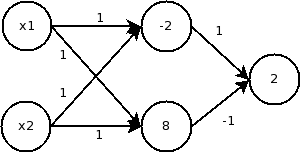
\includegraphics[width=.5\textwidth]{q7}
    \end{figure}
    
    For (-4,-4): both hidden nodes get a signal of -8, so both output negative 1. The weight on the bottom one is -1 though, 
    so the net input to the output node is 0, and it outputs -1. 
    
    For (-1,-1): both hidden nodes get a signal of -2, so the top one outputs 1 and the bottom outputs -1. 
    the net input to the output node is 2, and it outputs 1. 
    
    For (1,1): both hidden nodes get a signal of 2, so the top one outputs 1 and the bottom outputs -1. 
    the net input to the output node is 2, and it outputs 1. 
    
    For (4,4): both hidden nodes get a signal of 8, so the top one outputs 1 and the bottom outputs 1. 
    the net input to the output node is 0, and it outputs -1. 
\end{document}